\documentclass{amsart}

\usepackage{amsmath}
\usepackage{cite}
\usepackage{graphicx}
\usepackage{url}
\usepackage{color}

\newtheorem{theorem}{Theorem}
\newtheorem{lemma}{Lemma}
\newtheorem{corollary}{Corollary}
\newtheorem{proposition}{Proposition}
\newtheorem{example}{Example}
\newtheorem{definition}{Definition}
\newtheorem{observation}{Observation}

\newcommand{\RR}{\mathbb R}
\newcommand{\fS}{\mathfrak S}

\newcommand{\aut}{\mathcal A}
\newcommand{\pairing}{\mu}
\newcommand{\ptangle}{\mathsf{X}}
\newcommand{\tangle}{\mathsf{Y}}
\newcommand{\ltangle}{\mathsf{L}}
\newcommand{\ccollection}{\mathsf{C}}

% arxivness
\newcommand{\arxiv}[1]{#1}
\newcommand{\notarxiv}[1]{}

% notes
\definecolor{violet}{rgb}{0.730,0.555,0.769}
\definecolor{purple}{rgb}{0.459,0.109,0.538}
\definecolor{grey}{rgb}{0.4,0.4,0.4}
\newcommand{\LB}[1]{\colorbox{yellow}{Lola: #1}} % feel free to customize!
\newcommand{\EM}[1]{\colorbox{violet}{\textcolor{white}{Erick: #1}}}

\newcommand{\FIGspr}{\
\label{FIGspr}
\begin{figure}
  \arxiv{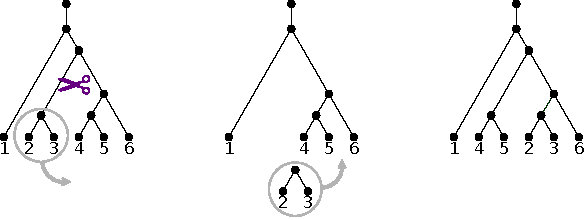
\includegraphics[width=4in]{figures/spr-definition}}
\caption{\
  A subtree-prune-regraft move.
}
\end{figure}
}

\newcommand{\FIGtanglegram}{\
\label{FIGtanglegram}
\begin{figure}
  \arxiv{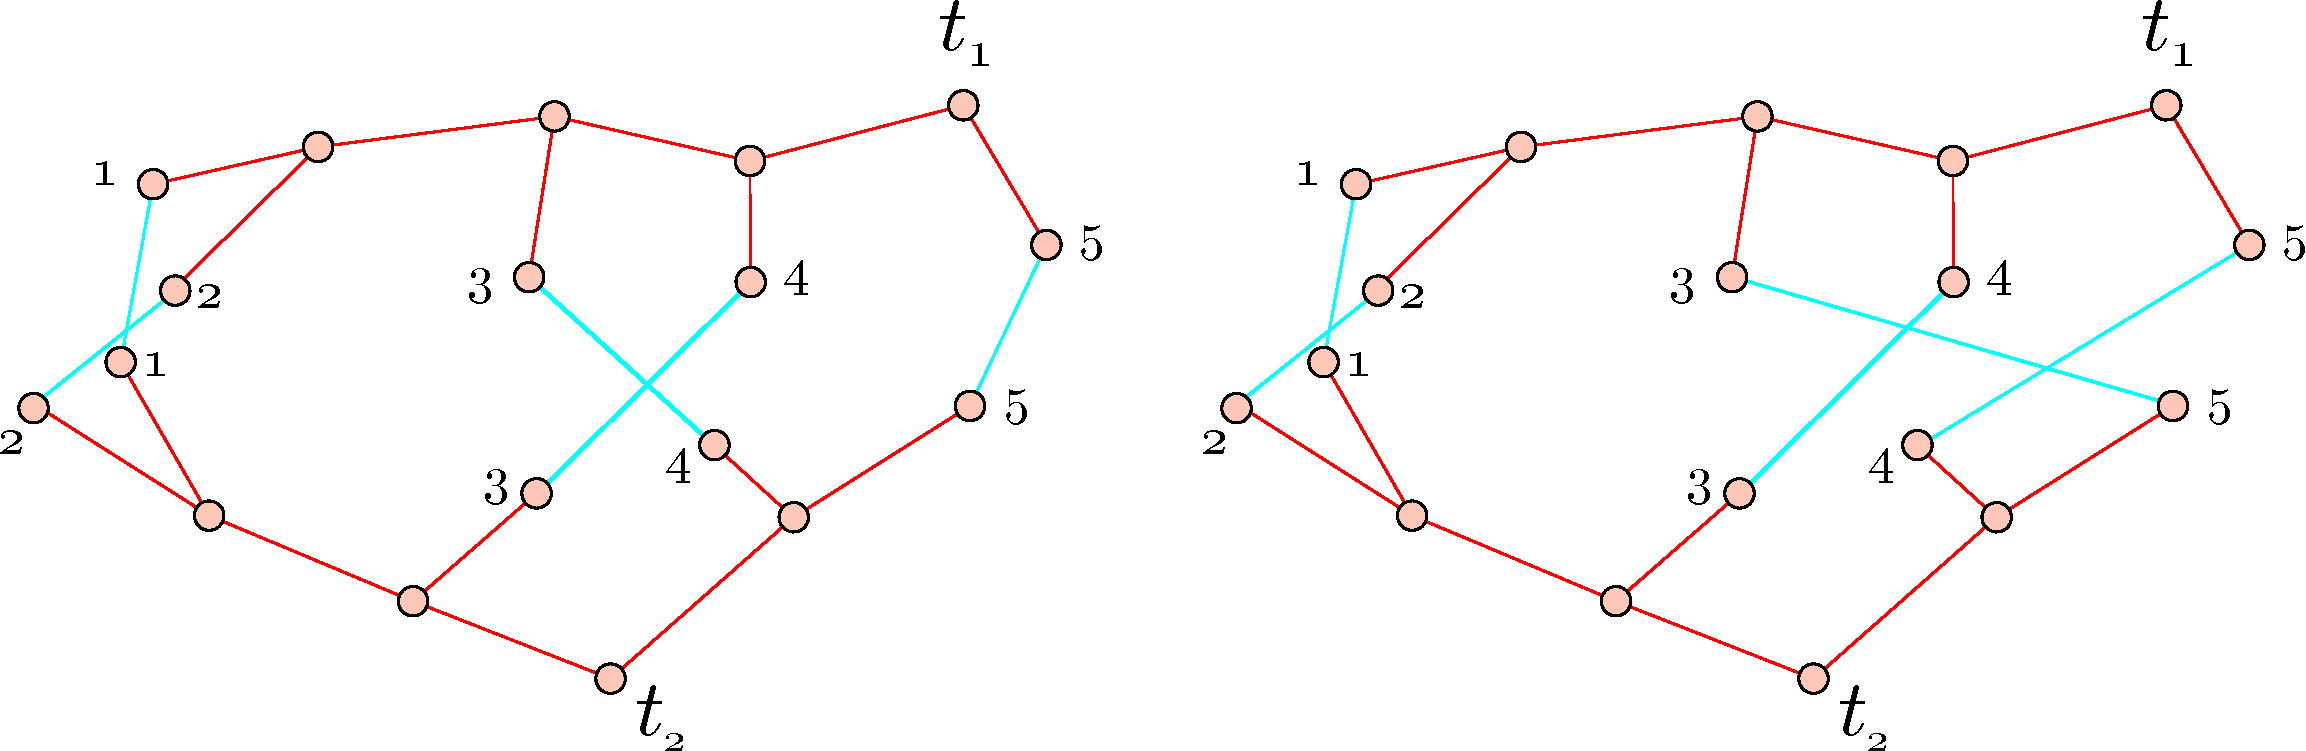
\includegraphics[width=5in]{figures/relabeling-example}}
\caption{\
  Two equivalent representations of the same tanglegrams.
  These two representations can be thought of as two planar embeddings of the same graph.
  Alternatively, they can be thought of as two permutations that are equivalent after taking symmetries of $t_2$ into account, or more formally two elements of the symmetric group which are equivalent under the action of the leaf automorphism group of $t_2$.
}
\end{figure}
}


\begin{document}
\title{Symmetries of tanglegrams}
\author[Matsen]{Frederick A. Matsen IV}
\address{Fred Hutchinson Cancer Research Center \\ Seattle, WA}
\thanks{Research supported in part by National Science Foundation award 1223057 and National Institutes of Health grant R01 GM113246-01}


\date{\today}

\begin{abstract}
Many interesting discrete mathematics problems concerning phylogenetic trees are defined in terms of the relative labeling of pairs of leaf-labeled trees.
These relative labelings are naturally formalized as so-called ``tanglegrams.''
Although there has been considerable work on planar embeddings of tanglegrams, many questions remain concerning their symmetries.
Understanding symmetries of tanglegrams would give information on how many problems on relatively labeled pairs of trees there are, open up the possibility for amortized algorithms, and reveal natural symmetries of spaces associated with such problems.
In this paper we develop methods to enumerate tanglegrams up to isomorphism, and we investigate the representation of the symmetric group induced by its action on tanglegrams.
\end{abstract}

\maketitle


\section{Introduction}
As a motivating example, we consider the problem of computing the \emph{subtree-prune-regraft} (SPR) distance between two leaf-labeled phylogenetic trees.
An SPR move cuts one edge of the tree and then reattaches the resulting rooted subtree at another edge (Figure~\ref{FIGspr}).
The SPR distance between two (phylogenetic, meaning leaf-labeled) trees $l_1$ and $l_2$ is the minimum number of SPR moves required to transform $l_1$ into $l_2$.
\FIGspr

Clearly the distance between two such trees does not depend on the actual labels of $l_1$ and $l_2$.
For example, one could exchange numbers labeling the two trees with their corresponding taxonomic names.
Or one could simply permute the numerical labels of the leaf nodes, which would result in the same distance if the permutation was applied identically on both the starting and ending trees (and trees on the shortest SPR path between the two).
Furthermore, a path made by SPR moves made by intermediate trees between the two trees could also have its labels permuted in order to give a path between the trees with permuted leaf labels.
Thus, all problems like SPR distance [make more formal] do not concern the actual leaf labels as such, but rather use the leaf labels as markers that can be used to map leaves of one phylogenetic tree on to another: the problem and its solutions are actually defined in terms of a \emph{relative} leaf labeling.

Such discrete mathematics problems and objects defined in terms of pairs of labeled combinatorial objects are ubiquitous in computational biology.
In addition to SPR distances and their cousin distances formed by \emph{nearest-neighbor-interchange} and \emph{tree bisection and reattachment} \cite{wiki:treeRearrangement}, we have their corresponding biological questions concerning ``supertree'' reconstruction \cite{Whidden2014-ku} and reconciliation of gene transfer networks \cite{Boon2013-mc}.
Because such moves are used in both maximum-likelihood heuristic search and Bayesian Markov chain Monte Carlo (MCMC) tree reconstruction, the geometry of phylogenetic trees under such moves has substantial consequences in terms of phylogenetic tree reconstruction \cite{Whidden2014-yt}.

[Expound on what this symmetry means for graphs of trees, such as the SPR graph. gh-4]

Another line of inquiry in computational biology concerns species delimitation, which can naturally be phrased in terms of inference of a partition of labeled objects.
In an analogous way, scientists use MCMC to explore the posterior on such partitions \cite{Yang2010-kc}, and comparison of the results can be performed using distances between the partitions via distances such as \cite{Gusfield2002-il}.
These partitions can also be thought of as a certain type of leaf-labeled tree of height two (see description below), and thus they also form a problem concerning relative leaf labeling of phylogenetic trees.

The concept of a pair of phylogenetic trees with a relative leaf labeling can be formalized as the graph-theoretic notion of a \emph{tanglegram} (Figure~\ref{FIGtanglegram}).
A tanglegram is a pair of trees on the same set of leaves with matching leaves in the two trees joined by an edge. \cite{Venkatachalam2010-zh}.
There has been extensive work concerning tanglegrams, focusing on the problem of drawing them in a way that has minimum crossings \cite{Buchin2008-lc,Lozano2008-tp,Bansal2009-ni,Bocker2009-xl,Fernau2010-an,Venkatachalam2010-zh}.
\FIGtanglegram

In this paper we explore the mapping of pairs of plane-embedded trees into the set of tanglegrams and explore the action of the symmetric group on tanglegrams.
We characterize the isomorphism classes in terms of the symmetries of the two phylogenetic trees they contain.
Furthermore, tanglegrams are equipped with a natural action of the symmetric group on the leaf set, which we describe.
We use the SAGE \cite{SteinJoyner2005} and GAP \cite{GAP4} mathematics software to further explore these symmetries, resulting in tables of representatives of tanglegrams and their multiplicities, as well as the irreducible representations of the symmetric group defined by the action on tanglegrams.

We note that even if one was not interested in group-theoretic properties as such, and might instead just be interested in a unique list of tanglegrams, it would be worth using a group theoretic approach because comparing group cosets (defined below) is inherently faster than checking graph isomorphism.

\section{Formalism}
Define planar embedding of a phylogenetic tree.
We will say that two embedded phylogenetic trees are identical if they are identical in the plane.
We will say that they are isomorphic if they are graph isomorphic, which doesn't take planar embedding into account.

We will start with a notion of a \emph{planar} tanglegram, which is a slight simplification of the notion of a \emph{drawing} used by previous authors \cite{Venkatachalam2010-zh} which will be convenient for our purposes.
Let $\fS_n$ denote the symmetric group on $n$ items.
\begin{definition}
\label{def:ptanglegram}
A rooted (resp. unrooted) \emph{planar $n$-tanglegram} is an ordered triple $(p_1, p_2, \pairing)$ where $p_1$ and $p_2$ are rooted (resp. unrooted) trees with $n$ leaves embedded in the plane, and $\pairing \in \fS_n$.
Let $\ptangle_n$ denote the set of planar $n$-tanglegrams.
\end{definition}

In order to be able to uniquely describe elements of the symmetric group, we will use the convention that the first tree in planar tanglegrams is labeled counter-clockwise, and the second tree is labeled clockwise, so that they end up looking like so

\begin{verbatim}
     /-- 3        3 --\
p1   \            2 --/\   p2
      \/-- 2            \
       \-- 1        1 --/
\end{verbatim}

[Perhaps we always want to draw them in a vertical orientation?]

\begin{definition}
\label{def:tanglegram}
A rooted (resp. unrooted) $n$-\emph{tanglegram} is an ordered triple $(t_1, t_2, \phi)$ consisting of two non-leaf-labeled rooted (resp. unrooted) trees $t_1$ and $t_2$ and a bijection $\phi$ between the leaves of $t_1$ and the leaves of $t_2$.
Let $\tangle_n$ denote the set of $n$-tanglegrams.
\end{definition}
There is a graph realization of a tanglegram where every leaf of $t_1$ is connected via an edge to the corresponding leaf of $t_2$.
There is a clear 1-to-1 correspondence between tanglegrams under relabeling and their graph realization (assuming they are considered up to graph isomorphism) by joining leaves of $t_1$ with their corresponding leaves in $t_2$ under $\pairing$.
If the two trees are rooted, we assume that something is done to distinguish the root nodes from other nodes of the tree.

[Clarify what graph isomorphism means in this context.]

Note that our definition respects the order of $t_1$ and $t_2$ by considering $(t_1, t_2, \pairing)$ to be different than the tanglegram $(t_2, t_1, \pairing^{-1})$ when $t_1$ and $t_2$ are different graph theoretically.
We can also consider an unordered tanglegram, or \emph{utanglegram}, by identifying them.

One might also consider a notion of \emph{labeled $n$-tanglegram} $(l_1, l_2, \pairing)$ in which $l_1$ and $l_2$ are phylogenetic (leaf-labeled) trees on the leaf set $\{1, \ldots, n\}$, and $\pairing \in \fS_n$ as before.
Let $\ltangle_n$ denote the set of labeled $n$-tanglegrams.
This is perhaps the most natural definition in terms of phylogenetics.


\section{Tanglegram symmetries}
It will be straightforward to describe the symmetries of tanglegrams in terms of symmetries of the trees from which they are built.
We will use cycle notation for elements of the symmetric group, such as $(1\ 2) (3\ 4)$, which can be distinguished from phylogenetic trees in Newick format \cite{wiki:newick}, such as $((1,2),(3,4));$, because symmetric group elements do not have commas or a trailing semicolon.
In order to conform to the convention used in GAP \cite{GAP4} and hence by SAGE \cite{SteinJoyner2005}, \emph{we will use the leftmost first convention of writing products in the symmetric group.}
Thus, in cycle notation, $(1\ 2) (1\ 3) = (1\ 2\ 3)$.
We will correspondingly consider groups as acting on the right, such that the action of $x.(\sigma \tau)$ is $(x.\sigma) . \tau)$.

\begin{definition}
Given a (rooted) phylogenetic tree $t$ on $n$ leaves embedded in the plane, let $\aut(t) \subset \fS_n$ be its leaf automorphism group: given a leaf labeling of $t$, $\aut(t)$ are the elements $\alpha$ of $\fS_n$ such that relabeling $t$ according to $\alpha$ results in an isomorphic leaf labeled tree.
\end{definition}
Because every tree has at least one cherry (a subtree of size 2), the automorphism group of every tree has at least the symmetry of exchanging the two leaves of that cherry.

Such tree symmetries induce symmetries of planar tanglegrams.
Given two subgroups $J$ and $K$ of a group $G$, a \emph{double coset} $JgK$ for some $g \in G$ is the set of elements $\{jgk \mid j \in J, k \in K\}$.
In fact,
\begin{observation}
There is a well-defined injective map from $n$-tanglegrams to ordered triples $(t_1, t_2, C)$ where $C$ is a double coset of $\fS_n$ defined by taking an arbitrary planar embedding $(\tilde t_1, \tilde t_2, \pairing_\phi)$ of the tanglegram and mapping
\begin{equation}
\label{eq:cosetMap}
(t_1, t_2, \phi) \mapsto (t_1, t_2, \aut(t_1) \pairing_\phi \aut(t_2)).
\end{equation}
\end{observation}
This map is well defined because any $\pairing$ defined by an alternate planar embedding of the tanglegram only differs from the arbitrary embedding by elements of $\aut(t_1)$ and $\aut(t_2)$.
It is injective because any if any pair of planar tanglegrams $(\tilde t_1, \tilde t_2, \tilde \pairing)$ and $(\hat t_1, \hat t_2, \hat \pairing)$ map to the same element, it means that the trees are (graph theoretically) isomorphic, defining $\alpha_i \in \fS_n$ mapping the leaves of $\tilde t_i$ to those of $\hat t_i$; then $\tilde \pairing = \alpha_1 \hat \pairing \alpha_2^{-1}$ and thus they have the same double coset image under the mapping \eqref{eq:cosetMap}.

This map is thus a bijection onto its image, and so we will use the two representations interchangeably.
For example, we will refer often to the coset of a tanglegram.
Given an arbitrary numbering of the leaves of $t_1$, we can actually realize each element of the coset as an element of the corresponding symmetric group.
With labeling equivalences in mind, we will often express a given tanglegram as two leaf-labeled trees and an element of the symmetric group.
We note that the various planar embeddings of the tanglegram graph are equivalent to choices of representatives $\pairing'$ of the coset tanglegram (i.e.\ $\pairing'$ such that $\aut(t_1) \pairing' \aut(t_2) = C$) given a choice of numbering for $t_1$.

It is now straightforward to enumerate tanglegrams.
Start by enumerating a list of (graph-isomorphism-unique) trees, and for each ordered pair $t_1$ and $t_2$ on $n$ leaves calculating the ensemble of distinct cosets $C$ of the form $\aut(t_1) \pairing \aut(t_2)$ for $\pairing \in \fS_n$.
The tanglegrams are then the set of triples $(t_1, t_2, C)$.
We can also pick an arbitrary labeled tanglegram for every tanglegram as its representative; we will call this choice a canonical collection $\ccollection_n$.

Now, given a labeled $n$-tanglegram $(l_1, l_2, \pairing)$, we would like to be able to map it to an element of $\ccollection_n$.
For each of the $l_i$, there is a leaf relabeling $\sigma \in \fS_n$ such that
\begin{equation}
\label{eq:repMap}
(l_1 . \sigma, l_2 . \sigma, \sigma^{-1} \aut(l_1) \pairing \aut(l_2) \sigma)
\end{equation}
is an element of $\ccollection_n$.
Indeed, $\sigma$ is uniquely defined (up to an element of $\aut(l_1)$) just by considering the relabeling of $l_1$, and using that $\sigma$ there must be a unique such representative \eqref{eq:repMap}, noting that $\alpha^{-1} \aut(l_1) \pairing \aut(l_2) \alpha = \aut(l_1) \pairing \aut(l_2)$ for $\alpha \in \aut(l_1)$ by definition. [does this deserve a little more clarification?]

[gh-3: utanglegram]


\section{Action of the symmetric group}
We define the action of the symmetric group on tanglegrams as that induced by right multiplication on $\pairing$, i.e.\ for $\sigma \in \fS_n$ and $(t_1, t_2, \pairing) \in \tangle_n$,
\[
(t_1, t_2, \pairing) . \sigma := (t_1, t_2, \pairing \sigma).
\]
We can think about this as giving the leaf-to-leaf mapping obtained by reordering the \emph{image} of the pairing map, which are the leaves of $t_1$.
We also note that
\[
(t_1, t_2, \pairing) . (\pairing^{-1} \sigma \pairing)  := (t_1, t_2, \sigma \pairing).
\]




\section{Acknowledgements}
This manuscript was substantially shaped by discussions with Michael Landis, Arnold Kas, and Chris Whidden.

\bibliographystyle{unsrt}
\bibliography{tangle}


\notarxiv{
\section{Figure legends}
\FIGspr
\FIGtanglegram
}
\end{document}

